\section{Conceptual Framework}
\label{sec:conceptual_framework}

Estimating capacity utilization involves an accounting challenge: while actual output is directly observable in national accounts, the productive ceiling remains a latent variable. This identification problem connects to the classical critique of aggregate production functions. Rather than attempting to estimate physical laws of production or marginal productivities through neoclassical functions, I follow Shaikh's (2016) approach of recovering capacity from the long-run relation between aggregate output and the capital stock. Because this estimated path serves as the denominator for the capacity utilization index, the properties of the resulting series depend directly on the stability of the output--capital coefficient driving that relation. To analyze this capacity ceiling, I ground the relationship in an aggregate Leontief production structure with fixed input proportions, a standard baseline in political-economy models of growth and distribution.

\subsection{Production Function and Productive Capacities}
\label{subsec:coefficient_capacity_path}

The empirical validity of a capacity-utilization series depends directly on the stability of the parameter that generates the fitted capacity path. While \citet{Shaikh2016} avoids direct physical proxies, his empirical output--capital relation can be grounded in a classical Leontief production structure:
\begin{equation}
Y_t = \min \{ A_t L_t, \mu_t R^n_t K_t \},
\end{equation}
where $Y_t$ is aggregate output, $L_t$ is employment, $K_t$ is the capital stock, $A_t$ is labor productivity, $R^n_t$ is the normal capacity--capital ratio (capital productivity at normal capacity utilization, $Y^p_t / K_t$), and $\mu_t$ is capacity utilization. In a capital-constrained setting where labor is not binding due to the reserve army of labor, this relation simplifies to $Y_t = \mu_t R^n_t K_t$. Taking natural logarithms yields:
\begin{equation}
\ln Y_t = \ln K_t + \ln R^n_t + \ln \mu_t.
\end{equation}

This Leontief specification provides an aggregate representation of an institutionally mediated production process. At the plant level, the conversion of equipment $K_t$ into potential capacity ($Y^p_t = R^n_t K_t$) depends on machine speeds, shift patterns, and labor effort. The normal capacity--capital ratio $R^n_t$ evolves over time as firms adopt technical and organizational adjustments. Once potential capacity is established, realized output $Y_t$ is determined by capacity utilization $\mu_t$, which responds to effective demand. From this perspective, workplace bargaining and managerial discipline influence the maximum output extractable from a given stock of equipment, motivating the inclusion of institutional factors in empirical capacity models.

Isolating the long-run capacity path requires modeling the unobserved normal capacity--capital ratio ($\ln R^n_t$). \citet{Shaikh2016} specifies this ratio as a linear function of a deterministic time trend and the capital stock:
\begin{equation}
\ln R^n_t = bt + c \ln K_t.
\end{equation}

Substituting this specification into the logarithmic Leontief relation yields the estimable level equation:
\begin{equation}
y_t = a + bt + d\,k_t + \varepsilon_t,
\qquad d \equiv 1+c,
\end{equation}
where $y_t$ and $k_t$ denote the logarithms of unscaled output and capital, while $d$ represents the long-run output--capital elasticity. In this paper, I reinterpret $d$ as the unbalanced-growth transformation elasticity $\theta \equiv \partial \ln Y^p / \partial \ln K$. The intercept $a$ absorbs initial conditions and scaling differences, while the linear trend ($bt$) is conventionally interpreted as autonomous technical change. Whereas Shaikh focuses primarily on the cointegrating residuals $\hat{\varepsilon}_t$ as a measure of capacity utilization, this study examines the stability of the underlying long-run relation linking capital accumulation to productive capacity ($g_{Y^p} = \theta g_K$).

The fitted path of productive capacity follows directly:
\begin{equation}
\hat{y}^p_t = \hat{a} + \hat{b}t + \hat{d}\,k_t,
\end{equation}
and capacity utilization is constructed as the ratio of realized output to this fitted ceiling:
\begin{equation}
\ln \hat{\mu}_t = y_t - \hat{y}^p_t,
\qquad
\hat{\mu}_t = \frac{Y_t}{\hat{Y}^p_t}.
\end{equation}

Under this construction, the utilization series inherits its level, cyclical amplitude, and variance directly from the estimated parameter $\hat{d}$. If alternative single-equation specifications produce divergent estimates of $\hat{d}$, they generate contradictory trajectories for both potential capacity and capacity utilization. The empirical credibility of the resulting index therefore rests on whether $\hat{d}$ reflects a stable long-run relationship or varies with lag structures and deterministic controls.

\subsection{Laws of Algebra and Laws of Production}

The estimated elasticity $d$ serves as the transformation elasticity ($\theta \equiv \partial \ln Y^p / \partial \ln K$) that anchors Shaikh's (2016) profit-rate decomposition. Because his measures of the normal rate of profit depend on the constructed capacity--capital ratio, the empirical behavior of this decomposition depends on the stability of $\hat{d}$. While national accounting identities link these profit aggregates, they leave the behavioral process translating investment into productive capacity unspecified. Following Shaikh’s (1974) critique and the accounting-identity argument developed further by \citet{Felipe2005}, regressions estimated with aggregate value data may approximate accounting identities rather than identify underlying technological relations. I apply this identification concern to Shaikh’s capacity regression.

\citet{Shaikh1974} demonstrated that the high statistical fit of Cobb-Douglas regressions reflects the underlying value-added identity ($p_t Y_t \equiv W_t + P_t = w_t L_t + r_t K_t$) under relatively stable factor shares, rather than physical substitution. In the capacity framework, the output--capital ratio is linked by identity to the profit rate ($r_t$) and the profit share ($\pi_t$) via $Y_t / K_t \equiv r_t / \pi_t$. Taking logarithms yields:
\begin{equation}
y_t - k_t = \ln r_t - \ln \pi_t.
\end{equation}
When this relation is estimated across periods marked by shifting profit shares and distributive conflict, a deterministic trend $bt$ may absorb variation in distribution rather than autonomous technical progress. The coefficient $d$ must adjust to satisfy the identity, producing an apparently stable regression fit while masking underlying changes in the distribution of income.

Historical data for the US corporate sector (1947--2011) from \citet{Shaikh2016} illustrate this connection. While real gross value added grew at an average annual rate of 3.0\% and real gross capital stock grew at 4.1\% (or 3.3\% and 4.4\%, respectively, under Shaikh's published $P_y$ deflator), the output--capital ratio averaged 0.53 with substantial medium-run swings. These movements coincide with distinct phases in the rate of exploitation ($e_t = \text{NOScorp}_t / \text{ECcorp}_t$), which measures corporate profits relative to employee compensation. During the post-war expansion (1947--1973), the exploitation rate was high and relatively stable, averaging 0.319 (corresponding to a net profit share of 21.8\%). During the 1974--1982 stagflation transition, a sustained profit squeeze reduced the exploitation rate to an average of 0.256 (profit share of 18.5\%). In the neoliberal period (1983--2011), the exploitation rate recovered to an average of 0.286 (profit share of 20.1\%). Because Shaikh's bivariate ARDL specification excludes distribution, the estimated elasticity may average across these distinct distributive regimes, appearing stable only by omitting historical shifts in income shares.

Measurement choices in constructing the capital stock introduce an additional consideration. The gross capital stock series $K_t$, reconstructed via Shaikh's Generalized Perpetual Inventory Method (GPIM) to correct for retirement profiles, averages 99.6\% of the BEA current-cost measure over 1947--2005. The remaining discrepancy between GPIM and BEA measures may reflect unobserved variations in asset discard patterns, maintenance, or running hours. Classical measurement error in the capital stock under standard assumptions tends toward attenuation bias in single-equation estimates, though finite-sample effects in dynamic models cannot be signed unconditionally. I therefore interpret empirical estimates of $\theta$ with caution regarding specification sensitivity.

\subsection{Balanced vs. Unbalanced Growth: Accumulation Regimes and Capital Accumulation Instability}
\label{subsec:balanced_unbalanced_growth}

Marxian reproduction theory provides a benchmark of proportional accumulation, as formalized in different ways by \citet{Okishio2022} and \citet{Basu2022}. In those formulations, the problem is interdepartmental: reproduction depends on proportional relations among departments and on the material requirements of accumulation. I translate this disproportionality problem into a single-sector capacity framework by allowing the transformation elasticity between capital accumulation and productive-capacity growth to depart from unity. In this representation, $\theta = 1$ is the proportional-growth benchmark, while $\theta \neq 1$ captures persistent divergence between capital accumulation and capacity formation.

Within this scalar representation, relaxing the proportional-growth benchmark ($\theta = 1$) introduces an unbalanced-growth closure ($\theta \neq 1$), where capacity formation systematically diverges from capital accumulation. Table~\ref{tab:growth_regimes} defines the three resulting accumulation regimes.

\begin{table}[H]
\centering
\caption{Accumulation Regimes and the Productive-Capacity Relation}
\label{tab:growth_regimes}
\small
\begin{tabular}{@{}>{\raggedright\arraybackslash}p{3.2cm}>{\centering\arraybackslash}p{1.8cm}>{\raggedright\arraybackslash}p{4.2cm}>{\raggedright\arraybackslash}p{4.0cm}@{}}
\toprule
Regime & Parameter Condition & Long-Run Relation $(\hat{Y}^p,\hat{K})$ & System Tendency \\
\midrule
\midrule
Balanced Growth & $\theta = 1.0$ & Capital and capacity expand proportionally & Knife-edge baseline \\
Overaccumulation & $\theta < 1.0$ & Capital expands faster than productive capacity & Accumulation decelerates toward stagnation ($\hat{k}^* = 0$) \\
Excess Capacity & $\theta > 1.0$ & Productive capacity expands faster than capital & Accumulation accelerates without supply-side limits \\
\bottomrule
\end{tabular}
\caption*{\footnotesize Note: This table defines the theoretical regimes governing the system.}
\end{table}

This single-sector classification provides an analytical baseline while abstracting from inter-sectoral imbalances between Department~I (means of production) and Department~II (means of consumption). In this setup, disproportionality is characterized by the gap between capital accumulation and capacity expansion when $\theta \neq 1$. The dynamic implications of this scalar representation are derived below.

The dynamic tendencies of these regimes can be formalized through an ordinary differential equation governing the acceleration of the net growth rate of the capital stock ($\hat{k} \equiv \dot{K}/K$), where the gross investment rate is $I/K = \hat{k} + \delta$ (so zero gross investment corresponds to $\hat{k} = -\delta$) and the sign of $d\hat{k}/dt$ depends on $(\theta - 1)$ (full derivations appear in Appendix~\ref{app:acc_dynamics}). When $\theta < 1$ (overaccumulation), capital expands faster than capacity ($g_{Y^p} < g_K$), reducing normal capital productivity and causing net accumulation to decelerate toward the stable stagnation equilibrium at $\hat{k}^* = 0$. When $\theta > 1$ (excess capacity), capacity outpaces capital, inducing dynamic acceleration. Figure~\ref{fig:ode_phase_diagram} illustrates these phase dynamics for stylized parameter values ($\theta = 0.8$ and $\theta = 1.2$). In practice, macroeconomic adjustments---such as rising wages, debt limits, or capital devaluation---prevent indefinite acceleration or collapse, but the directional tendencies reflect the underlying value of $\theta$.

\begin{figure}[H]
\centering
\caption{Capital accumulation dynamics under unbalanced growth}
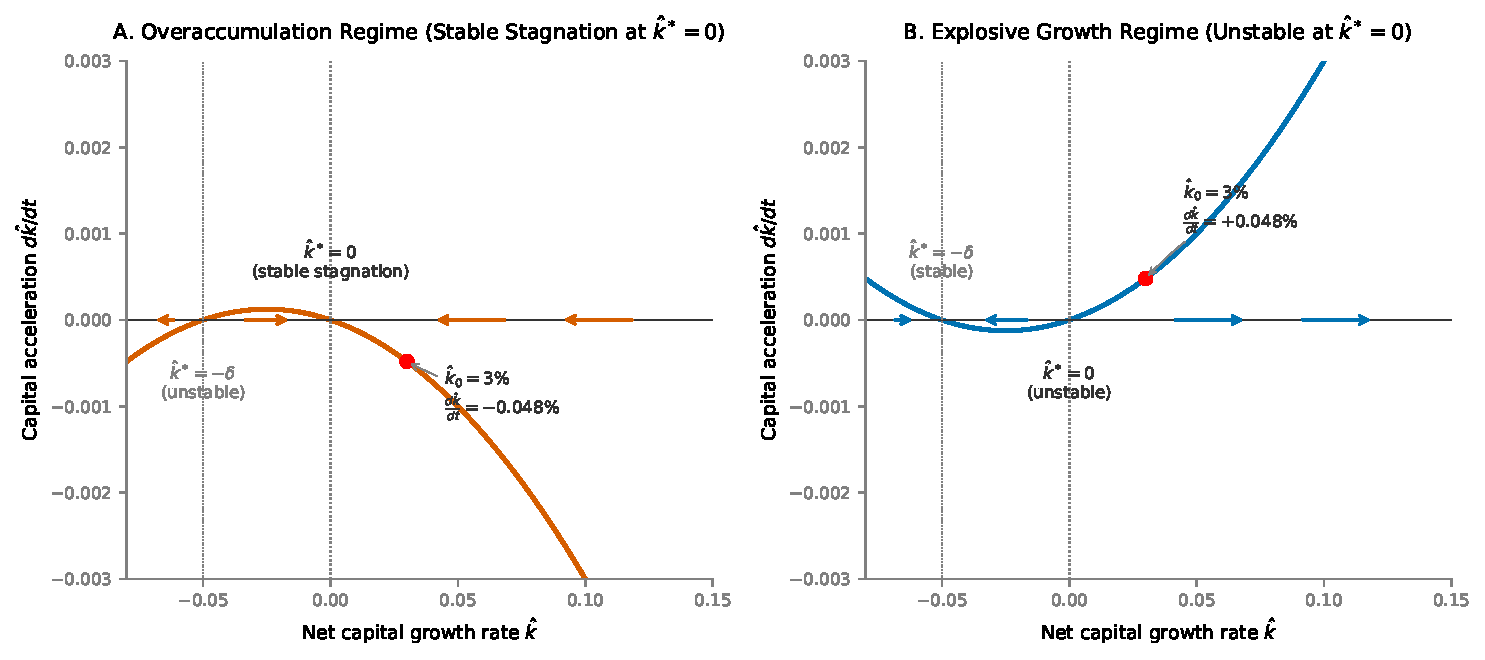
\includegraphics[width=0.92\linewidth]{figures/fig_S3_phase_diagram_capital_capacity_dynamics.pdf}
\caption*{\footnotesize Note: Panel A plots the overaccumulation regime ($\theta = 0.8 < 1.0$) where capital acceleration is negative for $\hat{k} > 0$ ($d\hat{k}/dt < 0$), pushing the net accumulation rate toward the stable stagnation equilibrium at $\hat{k}^* = 0$ (while $\hat{k}^* = -\delta$ represents the unstable lower boundary). Panel B plots the explosive growth regime ($\theta = 1.2 > 1.0$) where capital acceleration is positive for $\hat{k} > 0$ ($d\hat{k}/dt > 0$), causing the accumulation rate to diverge from $\hat{k}^* = 0$. Both panels show the initial condition $\hat{k}_0 = 3\%$ where $d\hat{k}/dt = \mp 0.048\%$, consistent with the numerical example in \S\ref{subsec:balanced_unbalanced_growth}.}
\label{fig:ode_phase_diagram}
\end{figure}

\subsection{Trend Stabilization, Viability Condition, and the Double-Misspecification Bias}
\label{subsec:trend_stabilized_closure}

Introducing a deterministic time trend ($b$) into the unbalanced growth closure ($g_{Y^p} = \theta g_K + b$) alters the dynamic properties of the system. Substituting this closure into the acceleration equation produces a quadratic differential equation:
\begin{equation}
\frac{d\hat{k}}{dt} = (\hat{k} + \delta)\left[(\theta - 1)\hat{k} + b\right].
\end{equation}
Under overaccumulation ($\theta < 1$) with positive technical progress ($b > 0$), this specification creates a locally stable interior steady state:
\begin{equation}
\hat{k}^* = \frac{b}{1 - \theta}.
\end{equation}
The ratio $b / (1 - \theta)$ balances autonomous technical progress against the drag of overaccumulation, preventing the net accumulation rate from falling to zero (as detailed in Appendix~\ref{app:acc_dynamics}).

However, treating this trend-stabilized path as an exogenous technical baseline is conceptually problematic. Following \citet{Basu2022}, technical change under capitalism is constrained by capitalist viability: profit-seeking firms adopt new techniques only if they reduce unit production costs at prevailing wages and input prices. The direction of technical change---whether capital-using and labor-saving or capital-saving and labor-saving---is endogenously shaped by class conflict over the real wage relative to labor productivity. Consequently, a deterministic time trend ($bt$) in the capacity regression does not capture neutral technical progress; it acts as an econometric sponge that absorbs the cumulative effects of distributional conflict and induced technical change.

This setup creates a risk of compound misspecification in econometric estimation. As \citet{Basu2020} emphasizes, when an empirical model omits a relevant variable---such as distribution influencing the choice of technique \citep{Kurz1986}---while including an exogenous proxy such as a deterministic trend, the estimated coefficient on capital suffers from compound bias. The trend mathematically absorbs unobserved shifts in distribution, compromising the structural interpretation of the recovered elasticity $\theta$.

Furthermore, estimating this relation over a 64-year sample (1947--2011) assumes that $\theta$ and $b$ remain invariant across major structural shifts: the post-war boom (1947--1973), the stagflation transition (1974--1982), and the neoliberal era (1983--2011). Imposing fixed coefficients forces the model to average across distinct institutional and macroeconomic regimes.

Finally, this framework connects to theoretical debates on the endogeneity of investment. In Neo-Kaleckian models, capital accumulation adjusts endogenously to demand-induced utilization gaps, whereas Sraffian supermultiplier models treat investment as anchored in autonomous demand components and cost-minimizing technique choices. Examining whether capital accumulation responds to long-run capacity disequilibria provides an empirical test of these alternative adjustment mechanisms. The subsequent empirical sections implement this replication and testing strategy.
